\section{Scene and objects description}

\begin{figure}[ht]
    \centering
    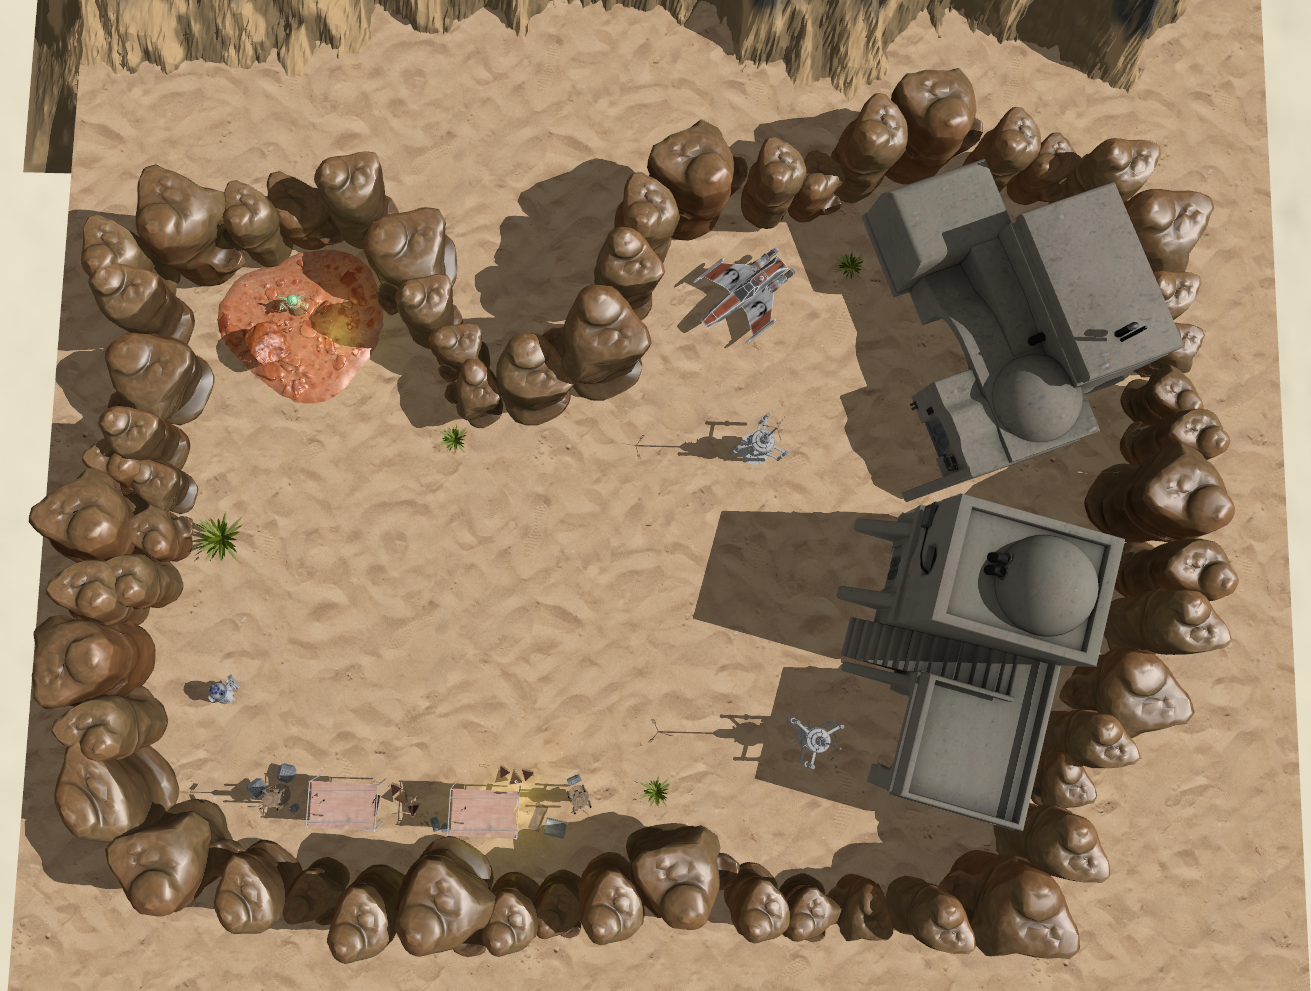
\includegraphics[width=\linewidth]{img/top_view.png}
    \caption{View of the scene from the top}
    \label{fig:top}
\end{figure}

The application uses two \textbf{skyboxes}. For daytime it uses a skybox showing a desert with mountains (Figure \ref{fig:skybox_day}) and for nighttime it uses one which presents a starry sky (Figure \ref{fig:skybox_night}).

The directional light source of the application is the \textbf{sun}, which can be rotated around an \textit{arbitrary axis}. The axis is hard-coded, however it can be changed by modifying a global constant. (Figure \ref{fig:skybox_day}). The skybox also contains a sun at the top. Hovewer it is not a mistake because Tatooine is part of a binary solar system i.e. there are two suns.

Since the scene presents a desert planet, the \textbf{ground} should be covered in sand. This was achieved by mapping a sand texture to a wide, slim rectangular box.

The scene is enclosed by \textbf{boulders}, forming a wall. It serves the purpose of increasing the photorealism by not allowing the user to directly see the skybox. Another important role of them is to block the camera from exiting the scene.

Next to the scene a small \textbf{mountain} is placed which helps building a more realistic view in the distance. In some positions its peak hides the sun, thus projecting a reflection to the scene. (Figure \ref{fig:rock})

In this planet people obtain their daily supply of water by extracting the water molecules form the air. The so cold \textbf{moisture vaporators} have a great importance, thus the scene contains a few of them. (Figure \ref{fig:building})

The scene contains two \textbf{buildings} in the architectural style of the desert worlds. (Figure \ref{fig:building})

In front of the leftmost building, in the corner, one can find a \textbf{Jedi star-ship}. Their symbol is painted on it. When the Jedi knights have individual missions in foreign planets, they usually travel by similar ships, accompanied by only their astromech droid. These droids can repair the ship and can have conversation with their owner. The head of such droid can be seen in behind the pilot cabin. (Figure \ref{fig:ship})

As for any habitable planet, Tatooine has markets in its settlements. A \textbf{fruit stand} was placed in the scene, accompanied by seats, barrels, and other items which can give the viewer the feeling of the marketplaces of the desert planet, like Mos Espa. (Figure \ref{fig:fruit_stand})

A triplet of \textbf{fireflies} are placed above the red fruits, which illuminate the nearby objects with yellow color. The fireflies form a point light source and have the same color as their emitted light. (Figure \ref{fig:fruit_stand})

Next to the fruit stand one can find two comfortable \textbf{seats} with a drink table. These items represent the entertainment of a more elegant class of citizens. (Figure \ref{fig:seats})

\textbf{R2-D2}, the most famous droid in the saga is also present in the scene. He serves an important role in the saga, some consider him a main character. (Figure \ref{fig:r2-d2})

Finally, the most loved creature of the recent years is present in an animation. \textbf{Grogu} aka. \textbf{``Baby Yoda''} is a small 50 year old force sensitive child who became beloved by the fans after its appearance in ``The Mandalorian'' serial. By using the Force, he can do telekinesis and move objects. In this animation we can see him pointing his hand towards the rock, and moving it periodically up-down while also rotating it. (Figure \ref{fig:baby_yoda})

For special effects, a \textbf{fog} was created with sand color to imitate a \textbf{sandstorm} (Figure \ref{fig:fog}).

\begin{figure}
    \centering
    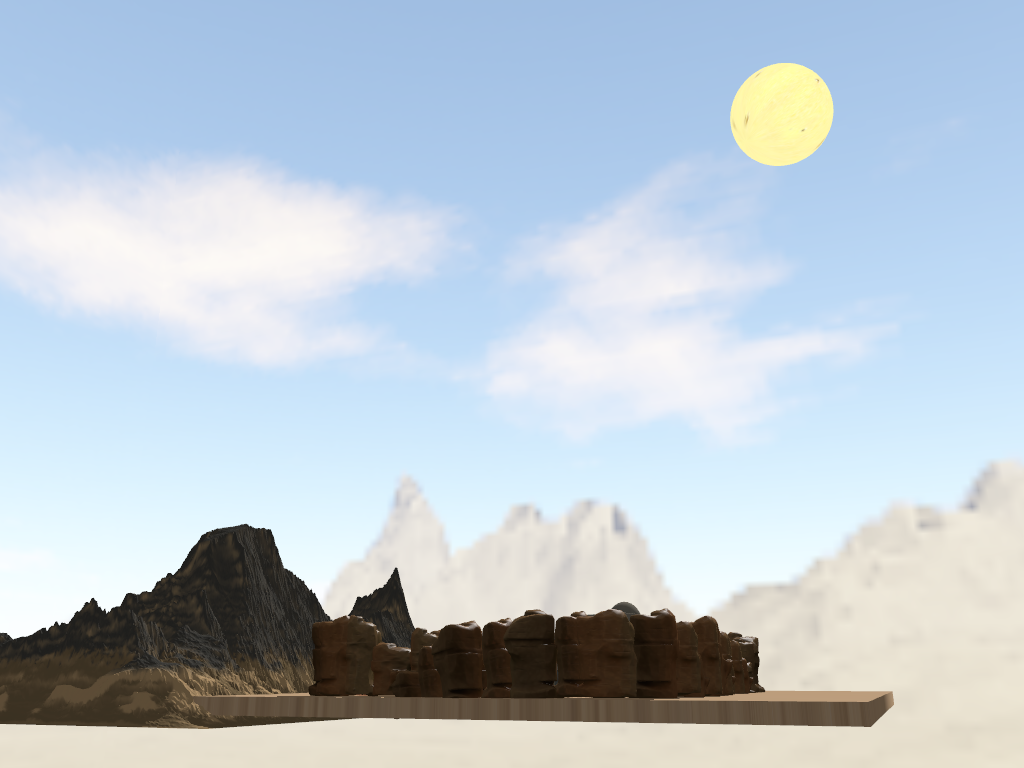
\includegraphics[width=.75\linewidth]{img/skybox_day.png}
    \caption{The scene and the sun enclosed by the daytime skybox}
    \label{fig:skybox_day}
\end{figure}

\begin{figure}
    \centering
    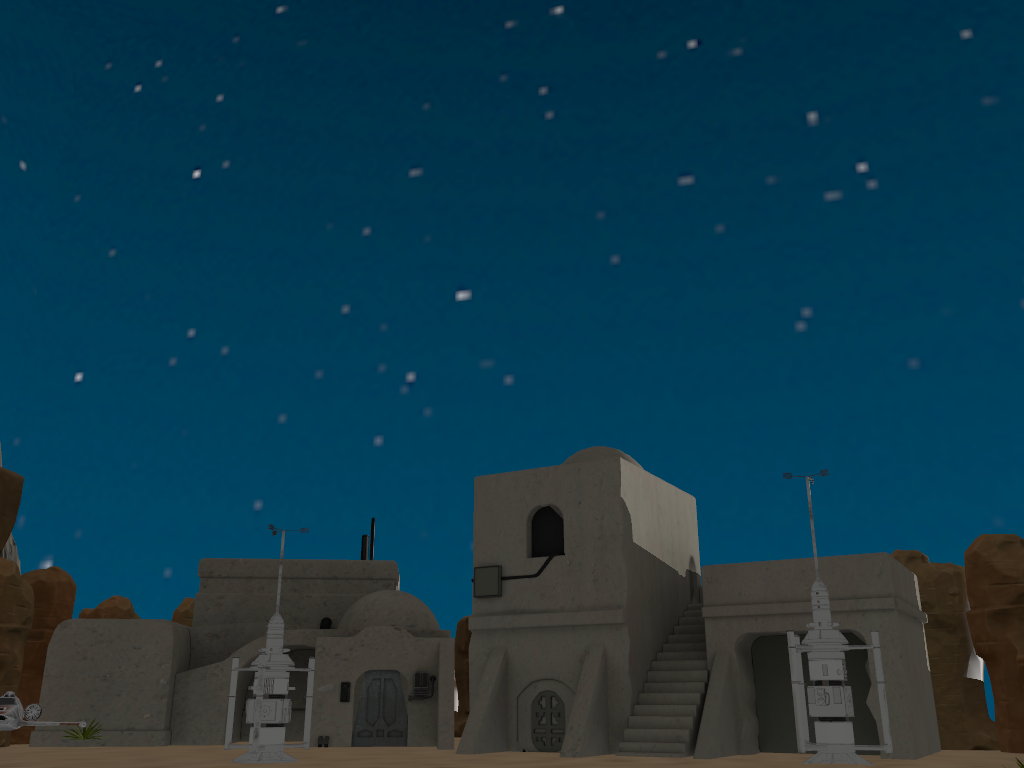
\includegraphics[width=.75\linewidth]{img/skybox_night.png}
    \caption{View of the sky at night}
    \label{fig:skybox_night}
\end{figure}

\begin{figure}
    \centering
    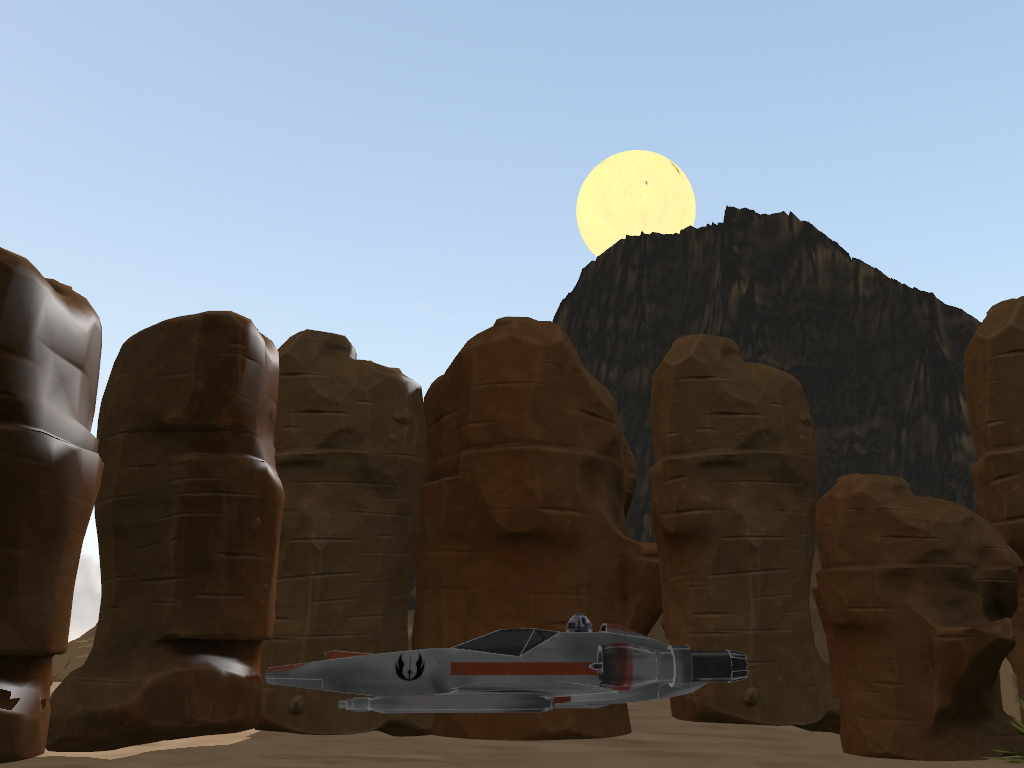
\includegraphics[width=.75\linewidth]{img/rock.png}
    \caption{View of the sun behind the peak of the neighboring mountain}
    \label{fig:rock}
\end{figure}

\begin{figure}
    \centering
    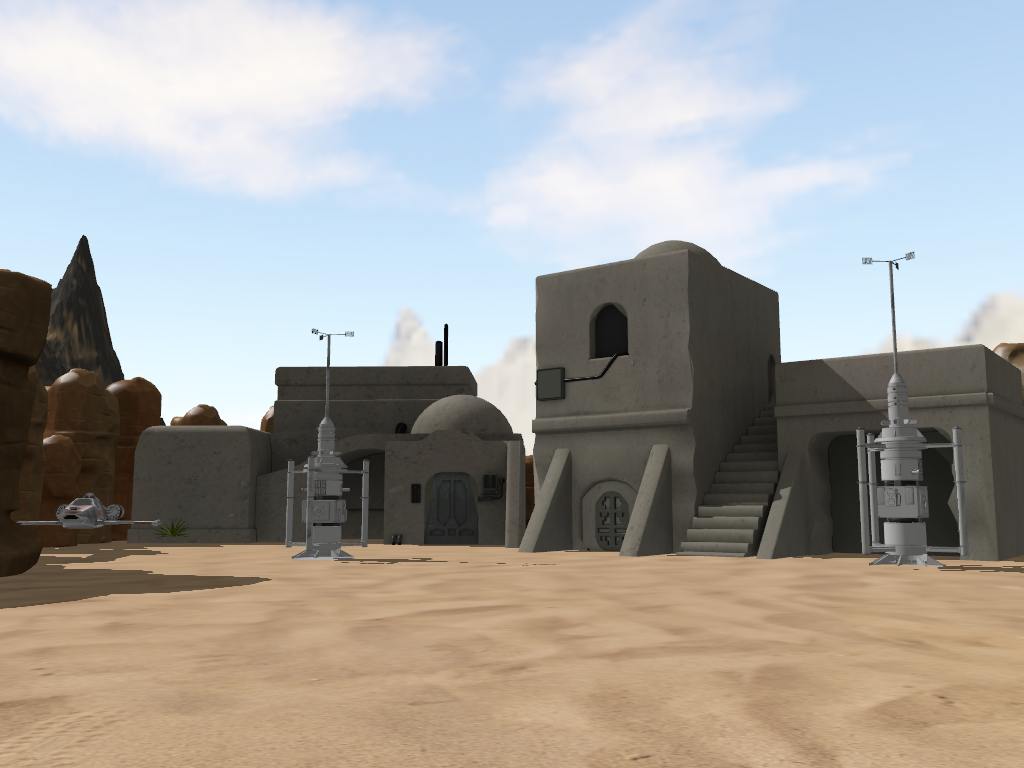
\includegraphics[width=.75\linewidth]{img/building.png}
    \caption{View of the moisture vaporators near the buildings in the morning}
    \label{fig:building}
\end{figure}

\begin{figure}
    \centering
    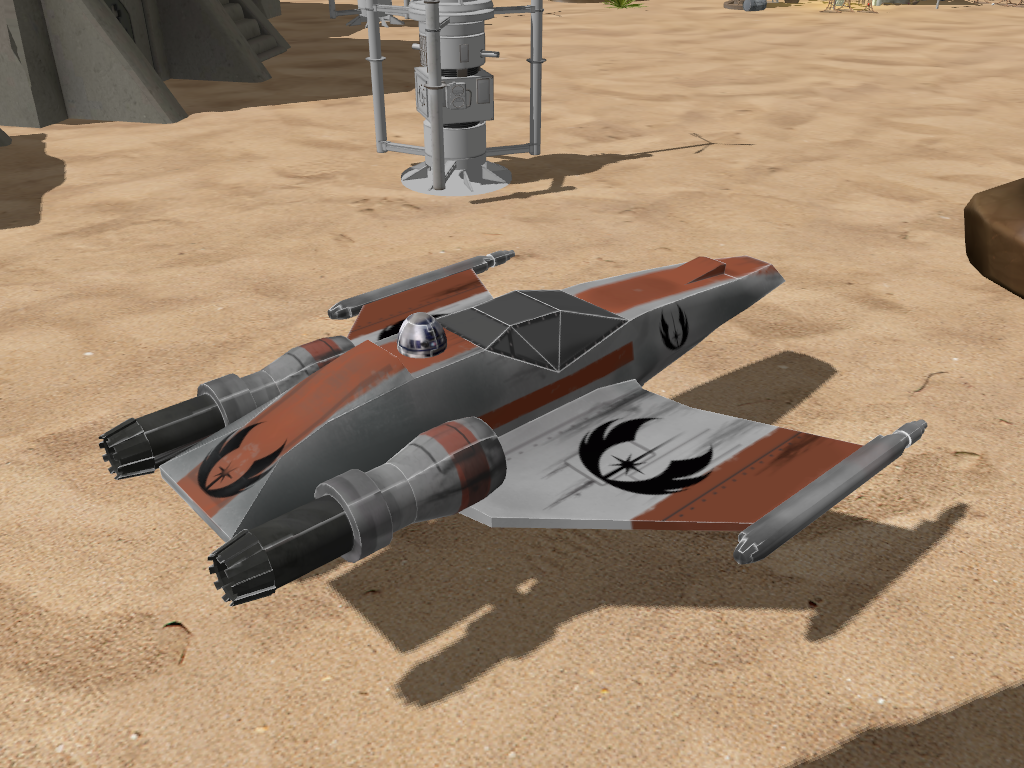
\includegraphics[width=.75\linewidth]{img/ship.png}
    \caption{View of the Jedi ship and its astromech droid}
    \label{fig:ship}
\end{figure}

\begin{figure}
    \centering
    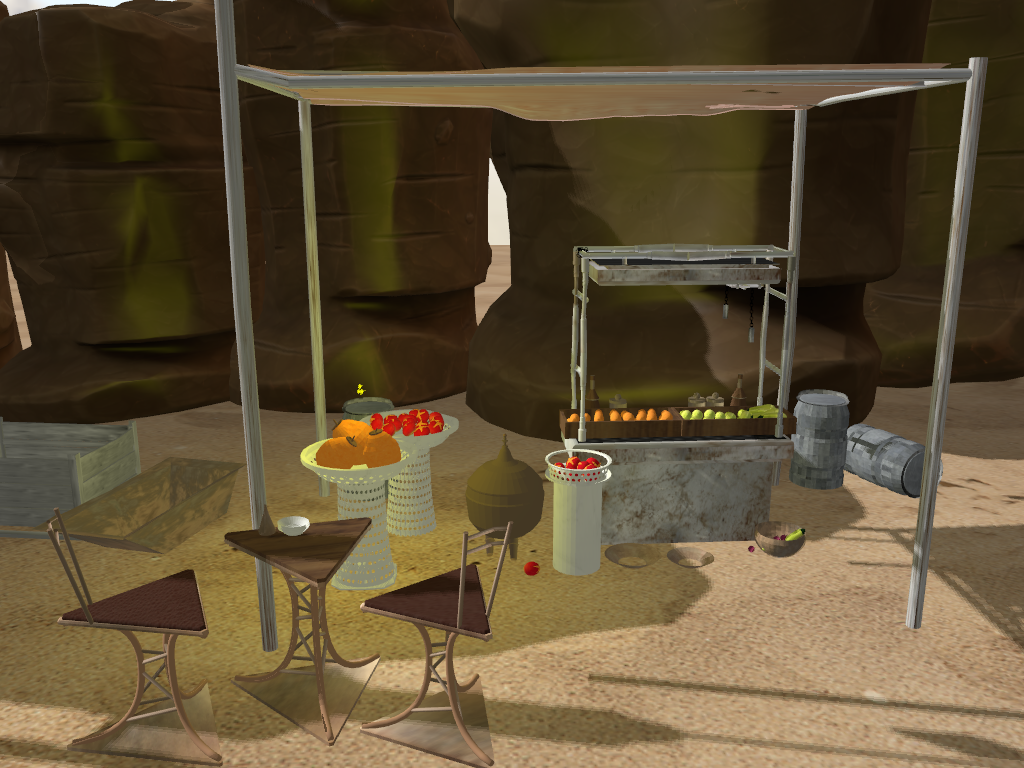
\includegraphics[width=.75\linewidth]{img/fruit_stand.png}
    \caption{View of the fruit stand before sunset, illuminated by the fireflies}
    \label{fig:fruit_stand}
\end{figure}

\begin{figure}
    \centering
    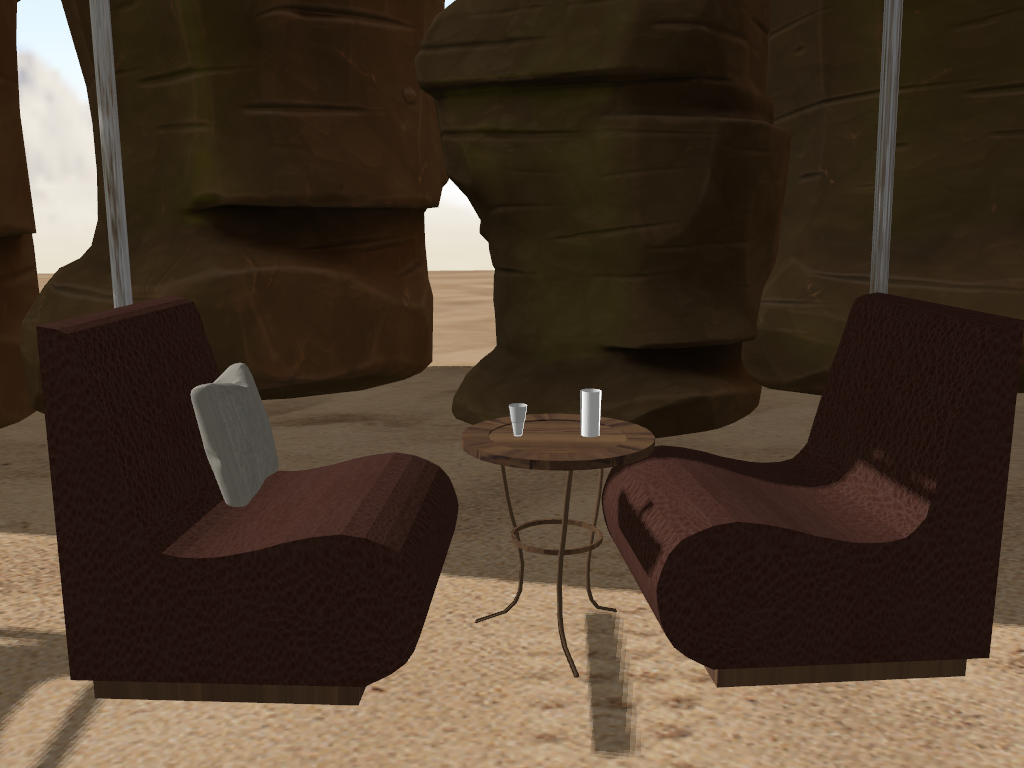
\includegraphics[width=.75\linewidth]{img/seats.png}
    \caption{View of two comfortable seats near a drink table}
    \label{fig:seats}
\end{figure}

\begin{figure}
    \centering
    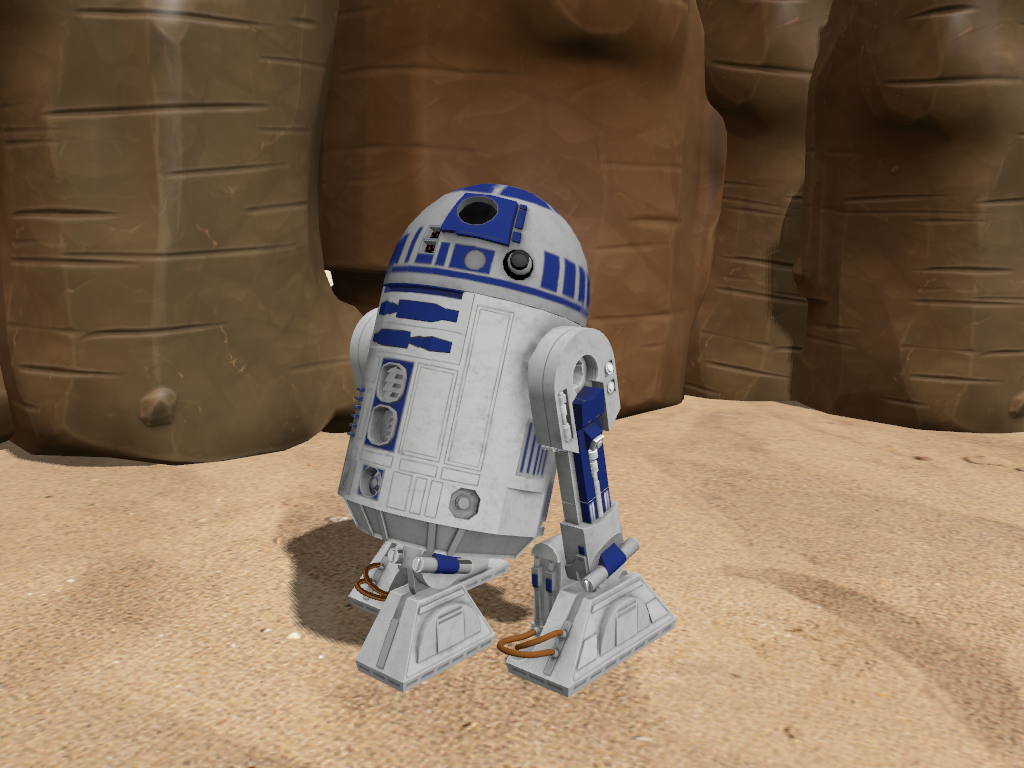
\includegraphics[width=.75\linewidth]{img/r2-d2.png}
    \caption{View of R2-D2 the favorite droid of the fans}
    \label{fig:r2-d2}
\end{figure}

\begin{figure}
    \centering
    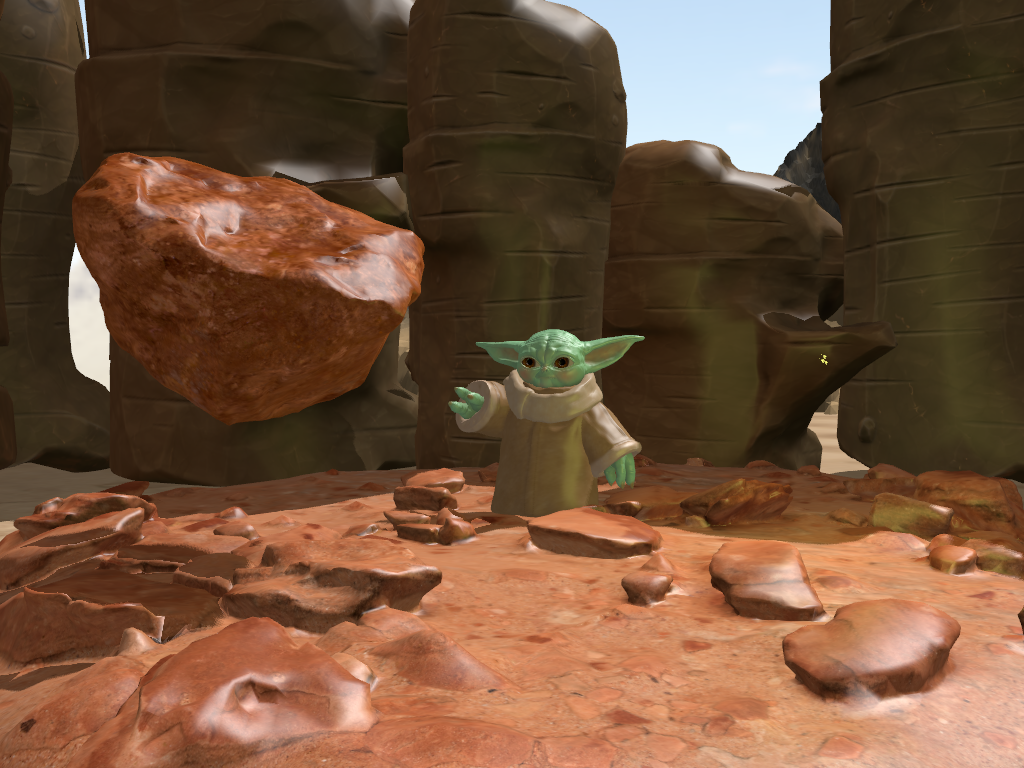
\includegraphics[width=.75\linewidth]{img/baby_yoda.png}
    \caption{View of ``Baby Yoda'' Grogu moving a rock using the force, illuminated by the sun and by fireflies}
    \label{fig:baby_yoda}
\end{figure}

\begin{figure}
    \centering
    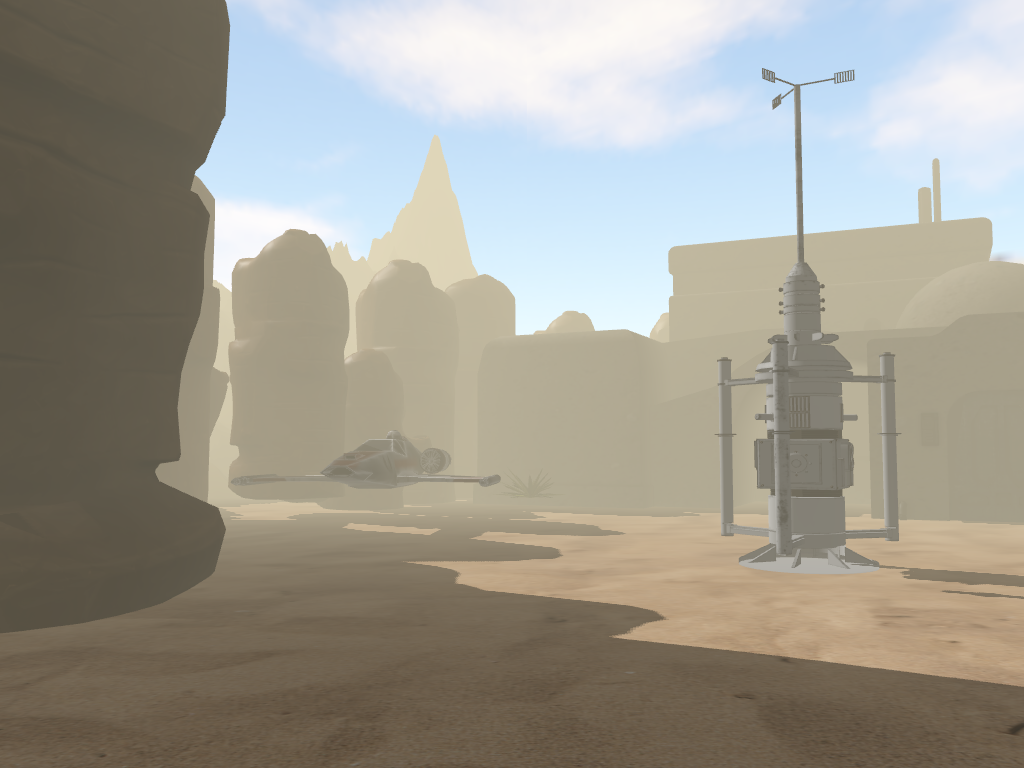
\includegraphics[width=.75\linewidth]{img/fog.png}
    \caption{View of a moisture vaporator in the sandstorm}
    \label{fig:fog}
\end{figure} 
